\documentclass{article}
\usepackage[utf8]{inputenc}
\usepackage{ upgreek }
\usepackage{graphicx}
\usepackage{ragged2e}
\usepackage[margin=2.5cm]{geometry}
\usepackage{array}
\usepackage{wrapfig}
\usepackage{multirow}
\usepackage{tabularx}
\usepackage{amsmath}
\usepackage{wrapfig}
\usepackage{mathtools}
\usepackage[table]{xcolor}
\usepackage{multirow}
\usepackage{polski}
\usepackage{rotating}
\usepackage{graphicx}
\usepackage{subcaption}

\title{Układy oscylacyjne}
\author{Marcin Gruchała 249882\\Jan Bronicki 249011\\}
\date{}

\begin{document}
\maketitle

\section{Cel ćwiczenia.}




Badanie odpowiedzi czasowej członu oscylacyjnego zgodnie z tabelą:
\begin{center}
\begin{tabular}{ |c|c|c|c| }
    \hline
    Przedział & Wybrana wartość $\xi$ & Wykres biegunów & Wykres skokowy \\ 
    \hline
    $\xi<-1$    & $-1.5$ & Rysunek \ref{fig:bieguny_ksi_-1_5}   & Rysunek \ref{fig:ksi_-1_5}\\
    \hline
    $-1<\xi<0$  & $-0.2$ & Rysunek \ref{fig:bieguny_ksi_-0_2}   & Rysunek \ref{fig:ksi_0_5}\\ 
    \hline
    $\xi=0$     & $0$    & Rysunek \ref{fig:bieguny_ksi_0}      & Rysunek \ref{fig:ksi_0}\\ 
    \hline
    $0<\xi<1$   & $0.5$  & Rysunek \ref{fig:bieguny_ksi_0_5}    & Rysunek \ref{fig:ksi_0_5}\\ 
    \hline
    $1<\xi$     & $1.5$  & Rysunek \ref{fig:bieguny_ksi_1_5}    & Rysunek \ref{fig:ksi_1_5}\\ 
    \hline
\end{tabular}

\end{center}




\section{Schemat.}
Schemat simulink:\\
 \begin{figure}[h!]
    \centering
    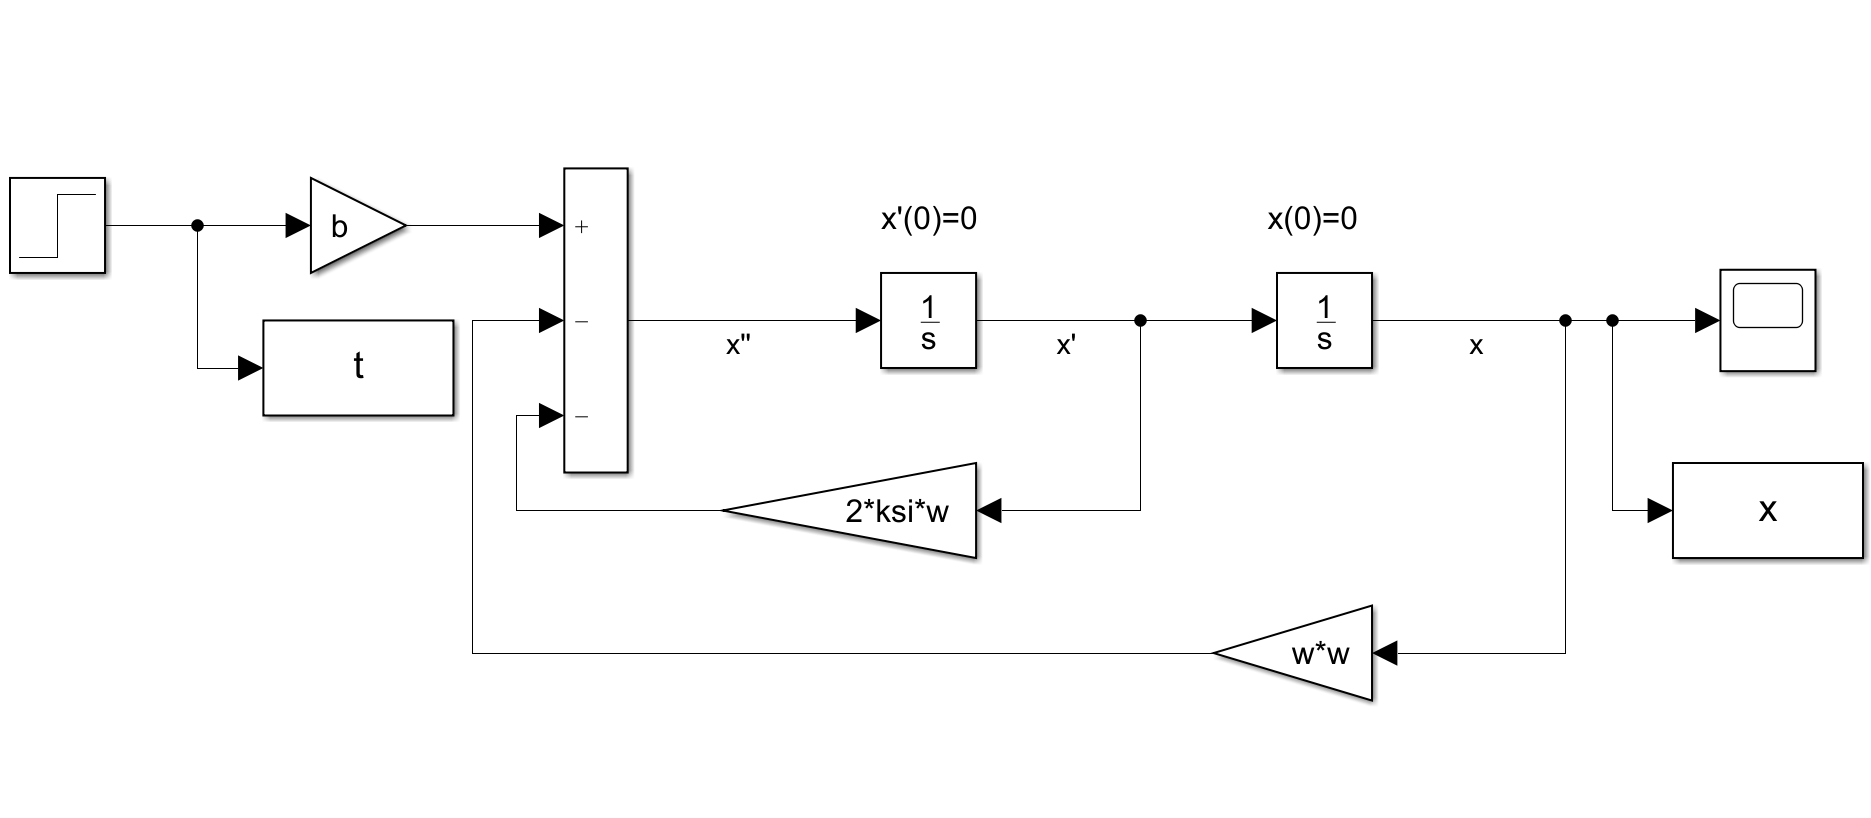
\includegraphics[scale=0.6]{schemat.png}
    \caption{Schemat simulinka}
    \label{fig:schemat}
 \end{figure}
 \newpage
 
\section{Wykresy rozwiązań.}


\begin{flushleft}
 a)  Przedział: $-1>\xi$, Wartość: $\xi=-1.5$\\
 
 
  Wykres biegunów:\\
 \begin{figure}[h!]
    \centering
    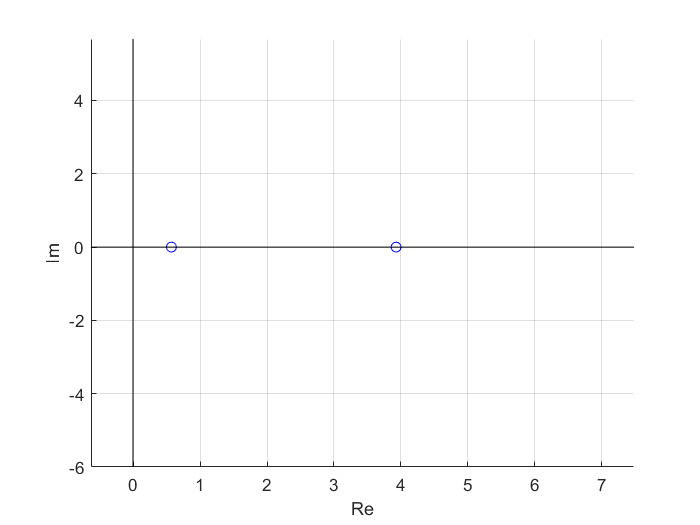
\includegraphics[scale=0.6]{bieguny_ksi_-1_5.png}
    \caption{Wykres biegunów, dla $\xi=-1.5$}
    \label{fig:bieguny_ksi_-1_5}
 \end{figure}
 
 
 Wykres odpowiedzi skokowej:\\
 \begin{figure}[h!]
    \centering
    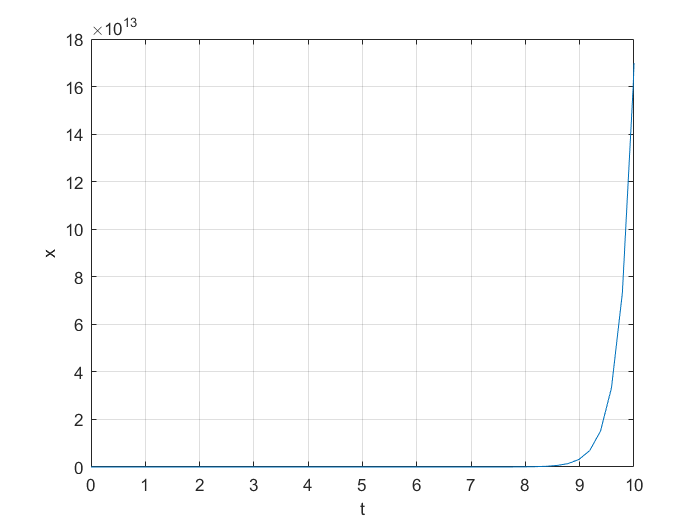
\includegraphics[scale=0.6]{ksi_-1_5.png}
    \caption{Wykres skokowy, dla $\xi=-1.5$}
    \label{fig:ksi_-1_5}
 \end{figure}
 
 
 \newpage
 b) Przedział: $-1<\xi<0$, Wartość: $\xi=-0.2$\\
  Wykres biegunów:\\
 \begin{figure}[h!]
    \centering
    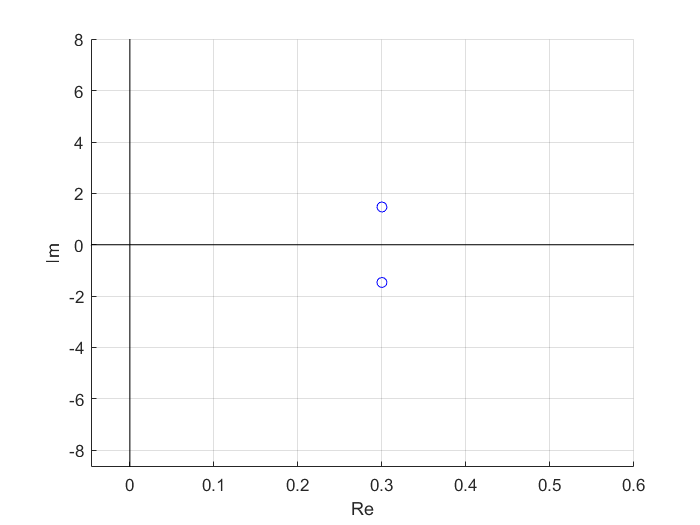
\includegraphics[scale=0.6]{bieguny_ksi_-0_2.png}
    \caption{Wykres biegunów, dla $\xi=-0.2$}
    \label{fig:bieguny_ksi_-0_2}
 \end{figure}
 
 
 Wykres odpowiedzi skokowej:\\
 \begin{figure}[h!]
    \centering
    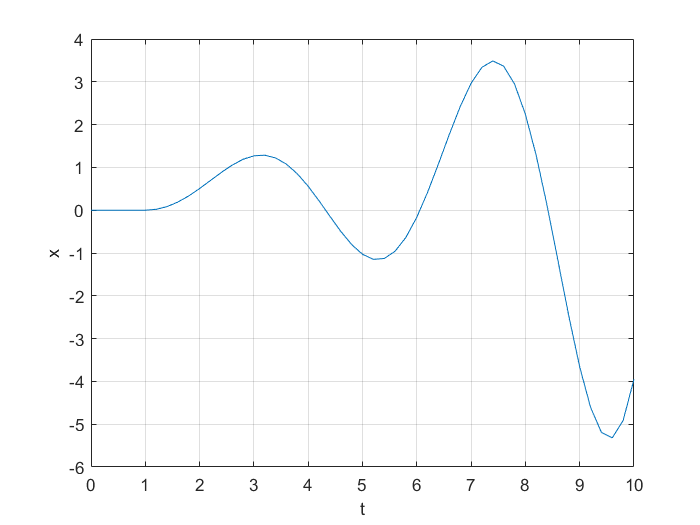
\includegraphics[scale=0.6]{ksi_-0_2.png}
    \caption{Wykres skokowy, dla $\xi=-0.2$}
    \label{fig:ksi_-0_2}
 \end{figure}
 
 \newpage
 c) Przedział: $\xi=0$, Wartość: $\xi=0$\\
 
 
 Wykres biegunów:\\
 \begin{figure}[h!]
    \centering
    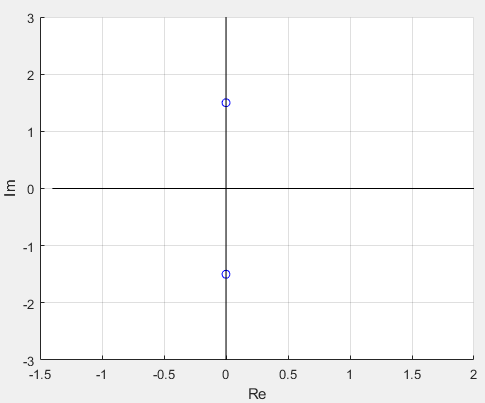
\includegraphics[scale=0.6]{biegunyksi0png.png}
    \caption{Wykres biegunów, dla $\xi=0$}
    \label{fig:bieguny_ksi_0}
 \end{figure}
 
 
 Wykres odpowiedzi skokowej:\\
 \begin{figure}[h!]
     \centering
    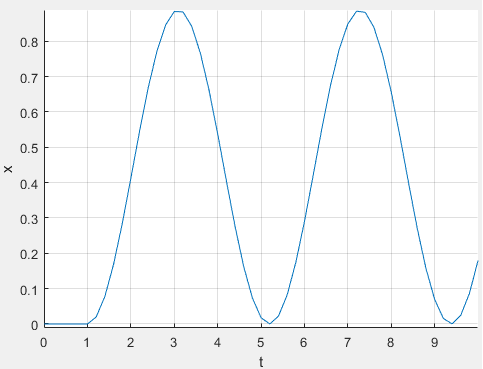
\includegraphics[scale=0.6]{skokksi0.png}
     \caption{Wykres skokowy, dla $\xi=0$}
     \label{fig:ksi_0}
 \end{figure}
 \newpage
 d)Przedział: $0<\xi<1$, Wartość: $\xi=0.5$\\
 
  Wykres biegunów:\\
 \begin{figure}[h!]
    \centering
    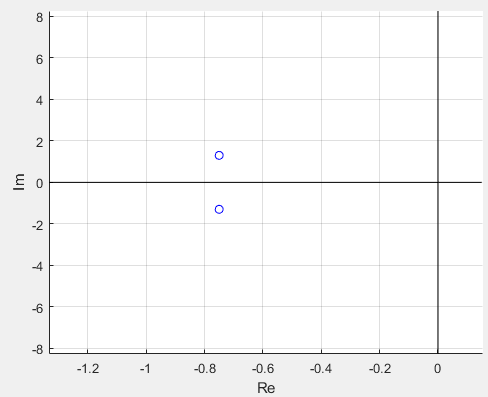
\includegraphics[scale=0.6]{biegunyksi05.png}
    \caption{Wykres biegunów, dla $\xi=0.5$}
    \label{fig:bieguny_ksi_0_5}
 \end{figure}
 

 Wykres odpowiedzi skokowej:\\
 \begin{figure}[h!]
    \centering
    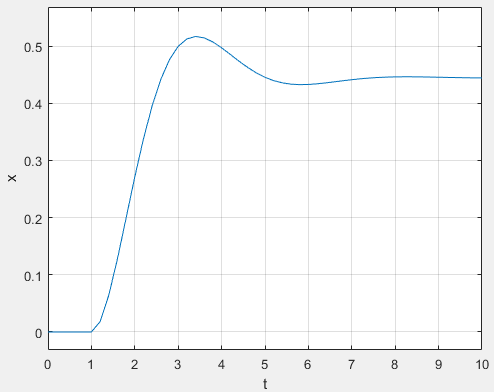
\includegraphics[scale=0.6]{skokksi05.png}
    \caption{Wykres skokowy, dla $\xi=0.5$}
    \label{fig:ksi_0_5}
 \end{figure}
 
 
 \newpage
 
 
 e) Przedział: $1<\xi$, Wartość: $\xi=1.5$\\
  Wykres biegunów:\\
 \begin{figure}[h!]
    \centering
    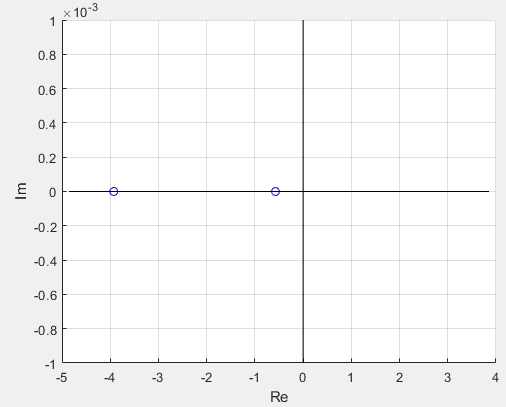
\includegraphics[scale=0.6]{biegunykis1,5.png}
    \caption{Wykres biegunów, dla $\xi=1.5$}
    \label{fig:bieguny_ksi_1_5}
 \end{figure}
 
 
 Wykres odpowiedzi skokowej:\\
 \begin{figure}[h!]
    \centering
    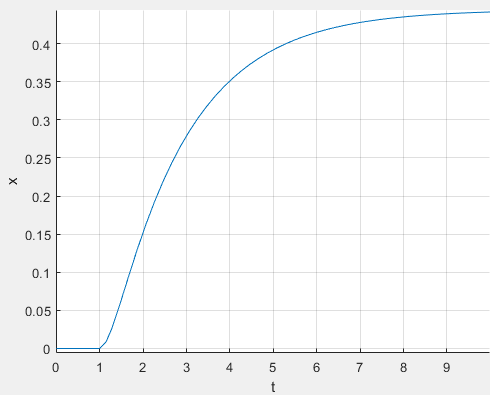
\includegraphics[scale=0.6]{skokksi1_5.png}
    \caption{Wykres skokowy, dla $\xi=1.5$}
    \label{fig:ksi_1_5}
 \end{figure}
\end{flushleft}

\section{Wnioski.}


\par Ćwiczenie pokazuje wpływ wartości współczynnika $\xi$ na równanie drugiego stopnia. Jak widać na wykresach po tym w jakim przedziale znajduje się $\xi$ można stwierdzić stabilność lub niestabilność układu.
\newpage
\section{Załączniki}

 \begin{figure}[h!]
    \centering
    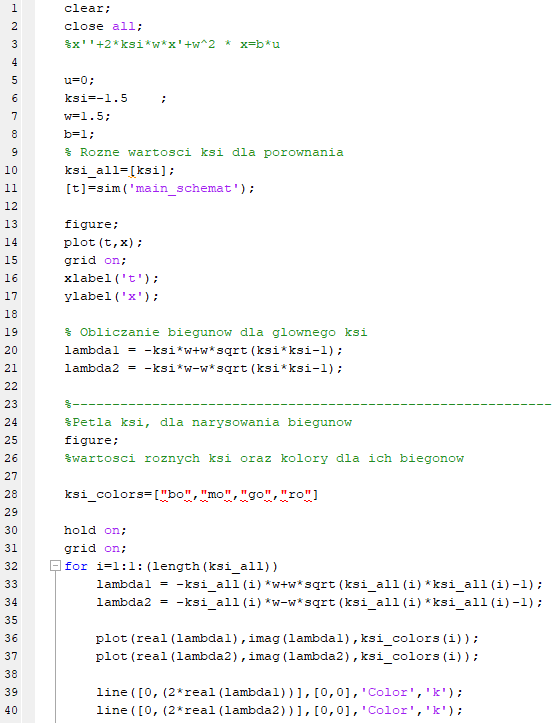
\includegraphics[scale=0.6]{kod1.png}
 \end{figure}
 
 \begin{figure}[h!]
    \centering
    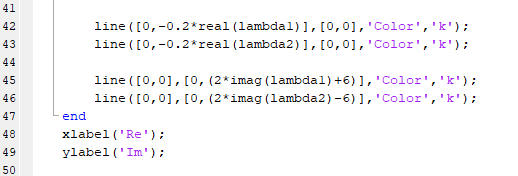
\includegraphics[scale=0.6]{kod2.png}
 \end{figure}







\end{document}
